\section{Story Maintenance}

Managing Stories
\newline
Stories for a project can easily be added, deleted and updated using murcS. To begin select 'Story' in the Display Choice picker (circled below)

\begin{figure}[H]
\centering
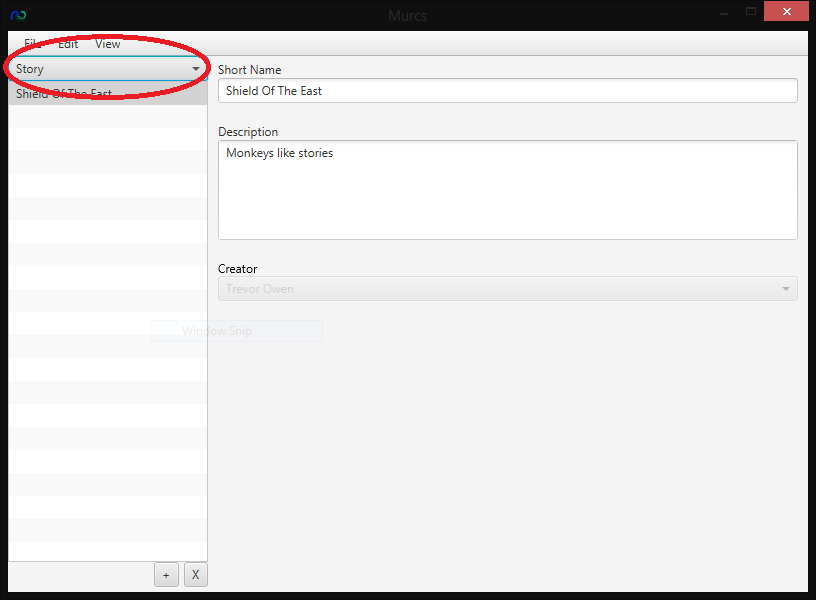
\includegraphics[width=\textwidth]{images/screenshots/stories1.PNG}
\caption{The Display Choice Picker}
\label{fig:new_project}
\end{figure}

Creating Stories
Stories can be created in two different ways, by clicking the add button (circled in red in the image below) or by navigating File-->New-->Story.

\begin{figure}[H]
\centering
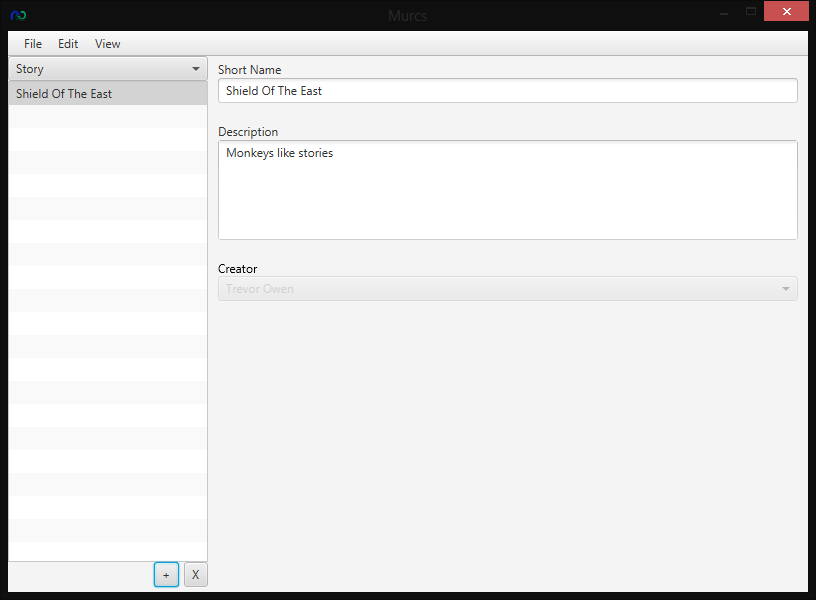
\includegraphics[width=\textwidth]{images/screenshots/stories2.PNG}
\caption{The Story Creation Dialog}
\label{fig:new_project}
\end{figure}

Whichever way you chose to create your story you will have been greeted with the following 'Story Creation Dialog' (pictured below). When creating a story you can specify a number of different fields. 

Name:
This is the name of your story. It must not be empty and must be unique, but you can change it later. This will show up in the display list, so make it recognizable!

Description:
To make life easier for your team it is helpful to know what a story is about. This is where the description field comes in. The description can be anything you like, but is most useful if it describes the story. You can change the description at any point.

Create:
This field stores the original creator of the story. It cannot be changed after the project has been created, so make sure you get it right first time.

\begin{figure}[H]
\centering
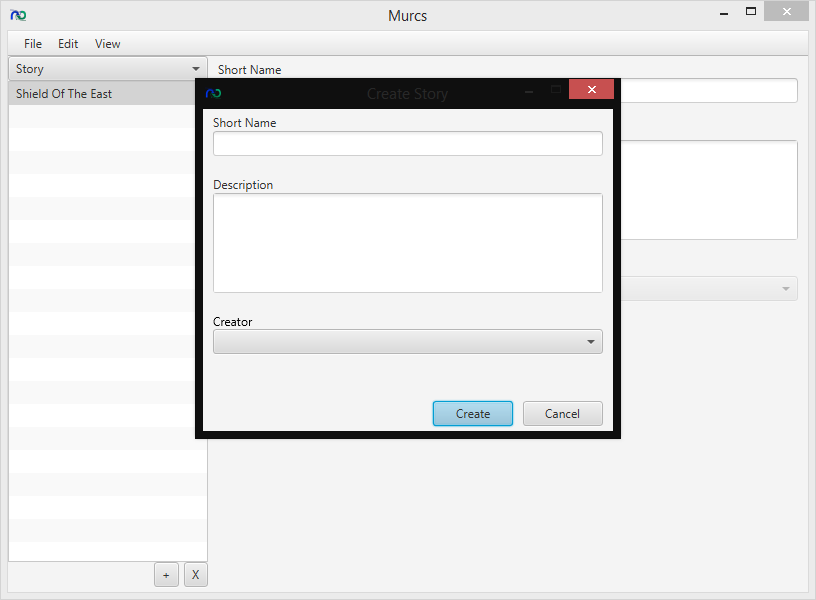
\includegraphics[width=\textwidth]{images/screenshots/stories3.PNG}
\caption{The Story Creation Dialog}
\label{fig:new_project}
\end{figure}

Updating
To update an existing story, simply select it from the display list. In the below picture we are editing the story known as 'Shield Of The East.' Note how the creator field is greyed out and cannot be changed.

\begin{figure}[H]
\centering
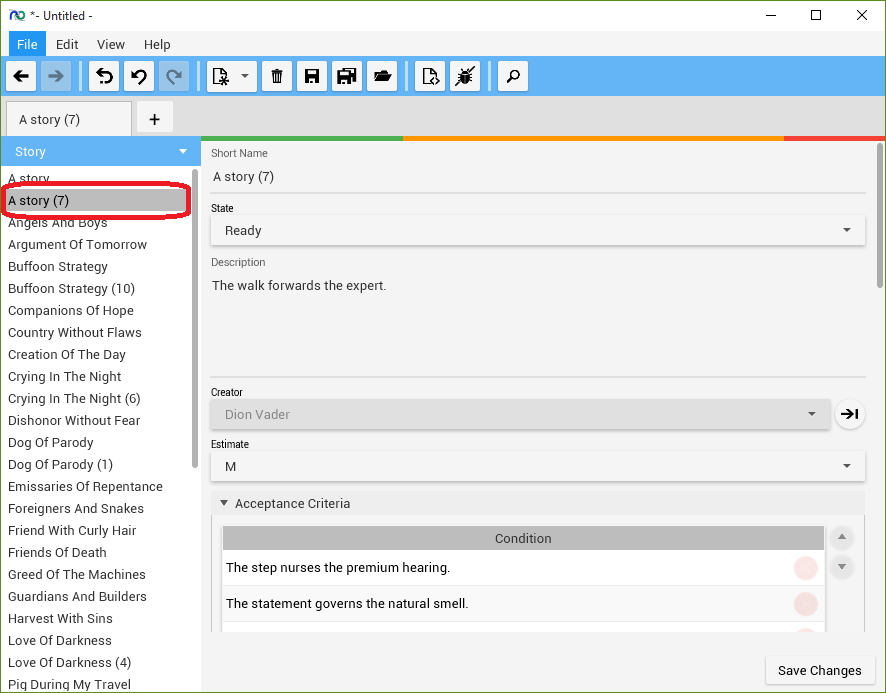
\includegraphics[width=\textwidth]{images/screenshots/stories4.PNG}
\caption{The Story Creation Dialog}
\label{fig:new_project}
\end{figure}

Deletion
To delete a story, simply press the 'X' button (circled below) at the bottom left of the screen, beneath the display list. You will be greeted with a confirmation dialog that will notify you of all the places the story is used. From this dialog you can go through with the deletion or cancel if you change your mind. For more information, see the 'Element Deletion' section of this guide.

\begin{figure}[H]
\centering
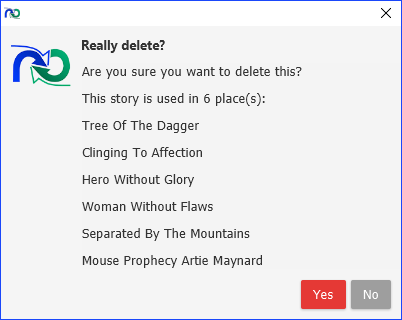
\includegraphics[width=\textwidth]{images/screenshots/stories5.PNG}
\caption{The Story Creation Dialog}
\label{fig:new_project}
\end{figure}